\documentclass[a4paper, 11pt]{article}
\usepackage[utf8]{inputenc}
\usepackage[T1]{fontenc}
\usepackage[polish]{babel}
\usepackage{graphicx}
\usepackage{amsmath}
\usepackage{amssymb}
\usepackage{geometry}
\usepackage{listings}
\usepackage{xcolor}
\usepackage{float} % Dla lepszego pozycjonowania tabel i obrazów
\usepackage{array} % Dla lepszych tabel

\geometry{a4paper, margin=1in}

% Definicja stylu dla MATLAB z polskimi znakami w komentarzach
\lstdefinestyle{matlab-polish}{
    language=Matlab,
    basicstyle=\ttfamily\small,
    keywordstyle=\color{blue},
    commentstyle=\color{green!40!black},
    stringstyle=\color{purple},
    showstringspaces=false,
    breaklines=true,
    frame=tb, % Ramka góra/dół
    captionpos=b, % Pozycja podpisu pod listingiem
    inputencoding=utf8, % Upewnij się, że plik wejściowy jest UTF-8
    literate={ą}{{\k{a}}}1 {ę}{{\k{e}}}1 {ć}{{\'c}}1 {ł}{{\l{}}}1 {ń}{{\'n}}1 {ó}{{\'o}}1 {ś}{{\'s}}1 {ź}{{\'z}}1 {ż}{{\.z}}1
             {Ą}{{\k{A}}}1 {Ę}{{\k{E}}}1 {Ć}{{\'C}}1 {Ł}{{\L{}}}1 {Ń}{{\'N}}1 {Ó}{{\'O}}1 {Ś}{{\'S}}1 {Ź}{{\'Z}}1 {Ż}{{\.Z}}1,
    morekeywords={optimoptions, ga}, % Dodaj specyficzne słowa kluczowe MATLABa
    numbers=left, % Numeracja linii
    numberstyle=\tiny\color{gray}, % Styl numeracji linii
    breakatwhitespace=false, % Łamanie linii tylko na białych znakach
    extendedchars=true, % Pozwala na polskie znaki w kodzie
}
\lstset{style=matlab-polish} % Ustawienie domyślnego stylu

\title{Algorytmy Ewolucyjne - Projekt 2 \\ Problem Plecakowy}
\author{Antoni Matczuk - 331129 \\ Jakub Szubzda - 331145} % Dane autorów
\date{\today}

\begin{document}
\maketitle
\newpage

\tableofcontents
\newpage

\section{Wstęp}
Celem projektu jest znalezienie rozwiązania problemu plecakowego przy użyciu algorytmu genetycznego. Problem plecakowy polega na wyborze takiego podzbioru przedmiotów spośród danego zbioru, aby suma wartości wybranych przedmiotów była jak największa, nie przekraczając jednocześnie określonego limitu wagowego plecaka. W ramach projektu wykorzystano środowisko MATLAB wraz z Global Optimization Toolbox.

\section{Definicja Problemu}
Problem plecakowy jest klasycznym problemem optymalizacyjnym. W wersji 0/1, dla każdego przedmiotu podejmujemy decyzję, czy zabrać go w całości, czy też nie. Matematycznie problem można sformułować następująco:

Maksymalizuj:
\[ \sum_{i=1}^{n} p_i x_i \]
Przy ograniczeniu:
\[ \sum_{i=1}^{n} w_i x_i \leq W \]
Gdzie:
\begin{itemize}
    \item $n$ - liczba dostępnych przedmiotów,
    \item $p_i$ - wartość $i$-tego przedmiotu ($p_i > 0$),
    \item $w_i$ - waga $i$-tego przedmiotu ($w_i > 0$),
    \item $x_i$ - zmienna decyzyjna, $x_i \in \{0, 1\}$ (1 jeśli przedmiot jest wybrany, 0 w przeciwnym razie),
    \item $W$ - maksymalna dopuszczalna waga plecaka.
\end{itemize}

\subsection{Generowanie Przedmiotów}
W ramach projektu zdefiniowano $n=32$ przedmiotów. Do ich generacji wykorzystano skrypt MATLAB, bazujący na Skrypcie 1 z treści zadania, używając numeru albumu `331129` (niższy numer albumu w przypadku pracy w parze).
\begin{itemize}
    \item Wagi przedmiotów ($w_i$) zostały wylosowane z rozkładem równomiernym z przedziału $\langle0.1, 1\rangle$ z dokładnością do 0.1.
    \item Wartości przedmiotów ($p_i$) zostały wylosowane z rozkładem równomiernym z przedziału $\langle1, 100\rangle$ z dokładnością do 1.
\end{itemize}
Maksymalna pojemność plecaka ($W$) została ustalona na 30\% sumarycznej wagi wszystkich przedmiotów. Suma wag wszystkich przedmiotów wynosi 17.4, zatem $W = 0.30 \times 17.4 = 5.22$.

\subsection{Lista Wszystkich Przedmiotów}
Poniższa tabela przedstawia listę wszystkich wygenerowanych przedmiotów wraz z ich wagami, wartościami oraz stosunkiem wartości do wagi.
\begin{table}[h!]
\centering
\begin{tabular}{|c|c|c|c|}
\hline
Nr & Waga & Wartość & Stosunek V/W \\
\hline
1 & 0.2 & 54 & 270.00 \\
2 & 0.2 & 86 & 430.00 \\
3 & 0.5 & 75 & 150.00 \\
4 & 0.6 & 83 & 138.33 \\
5 & 0.2 & 91 & 455.00 \\
6 & 1.0 & 91 & 91.00 \\
7 & 0.7 & 50 & 71.43 \\
8 & 0.6 & 9 & 15.00 \\
9 & 0.2 & 60 & 300.00 \\
10 & 0.8 & 48 & 60.00 \\
11 & 0.2 & 34 & 170.00 \\
12 & 0.7 & 23 & 32.86 \\
13 & 0.3 & 96 & 320.00 \\
14 & 1.0 & 83 & 83.00 \\
15 & 0.2 & 6 & 30.00 \\
16 & 0.4 & 33 & 82.50 \\
17 & 0.2 & 49 & 245.00 \\
18 & 0.8 & 50 & 62.50 \\
19 & 0.6 & 82 & 136.67 \\
20 & 0.7 & 8 & 11.43 \\
21 & 0.5 & 5 & 10.00 \\
22 & 1.0 & 69 & 69.00 \\
23 & 0.9 & 22 & 24.44 \\
24 & 0.7 & 84 & 120.00 \\
25 & 0.7 & 60 & 85.71 \\
26 & 0.8 & 11 & 13.75 \\
27 & 0.4 & 44 & 110.00 \\
28 & 0.8 & 50 & 62.50 \\
29 & 0.1 & 45 & 450.00 \\
30 & 0.5 & 10 & 20.00 \\
31 & 0.5 & 34 & 68.00 \\
32 & 0.4 & 49 & 122.50 \\
\hline
\end{tabular}
\caption{Lista wszystkich przedmiotów w problemie plecakowym}
\label{tab:all_items}
\end{table}


\newpage
\section{Algorytm Genetyczny}
Do rozwiązania problemu plecakowego wykorzystano algorytm genetyczny dostępny w MATLAB Global Optimization Toolbox.

\subsection{Funkcja Celu}
Funkcja celu algorytmu genetycznego została zdefiniowana jako minimalizacja negacji sumy wartości wybranych przedmiotów, co jest równoważne maksymalizacji sumy wartości:
\[ \text{fitnessFunction} = @(x) -\sum_{i=1}^{n} x_i \cdot \text{item\_values}_i \]
gdzie $x$ jest wektorem binarnym reprezentującym chromosom (wybór przedmiotów).

\subsection{Ograniczenia}
Jedyne ograniczenie dotyczy sumarycznej wagi wybranych przedmiotów, która nie może przekroczyć maksymalnej pojemności plecaka $W$:
\[ \sum_{i=1}^{n} x_i \cdot \text{item\_weights}_i \leq W_{max} \]
To ograniczenie zostało zaimplementowane jako ograniczenie nierówności liniowej `Aineq * x' <= bineq` w funkcji `ga`.

\subsection{Parametry Algorytmu Genetycznego}
Wybrane parametry algorytmu genetycznego użyte w symulacji to:
\begin{itemize}
    \item \textbf{Rozmiar populacji (PopulationSize):} 100
    \item \textbf{Liczba osobników elitarnych (EliteCount):} 5 (obliczone jako $\lceil 0.05 \times \text{PopulationSize} \rceil$)
    \item \textbf{Współczynnik krzyżowania (CrossoverFraction):} 0.8
    \item \textbf{Funkcja mutacji (MutationFcn):} {@mutationuniform, mutationRate}
    \item \textbf{Współczynnik mutacji (MutationRate):} 0.04
\end{itemize}

\subsection{Kryteria Zatrzymania Algorytmu}
Algorytm genetyczny kończył działanie po spełnieniu jednego z następujących kryteriów:
\begin{itemize}
    \item \textbf{Maksymalna liczba pokoleń (MaxGenerations):} 200
    \item \textbf{Liczba pokoleń bez poprawy (MaxStallGenerations):} 50
    \item \textbf{Tolerancja funkcji celu (FunctionTolerance):} 1e-7
\end{itemize}

\subsection{Konfiguracja Algorytmu w MATLAB}
Poniższy fragment kodu przedstawia konfigurację opcji dla algorytmu genetycznego w MATLABie:
\begin{lstlisting}[language=Matlab, caption={Konfiguracja opcji algorytmu genetycznego w MATLAB}, label={lst:ga_options}]
options = optimoptions('ga', ...
    'PopulationSize', populationSize, ...
    'EliteCount', eliteCount, ...
    'CrossoverFraction', crossoverFraction, ...
    'MutationFcn', {@mutationuniform, mutationRate}, ...
    'MaxGenerations', maxGenerations, ...
    'MaxStallGenerations', stallGenerations, ...
    'FunctionTolerance', functionTolerance, ...
    'Display', 'off', ...
    'PlotFcn', {}, ... % Wykresy generowane przez OutputFcn
    'OutputFcn', @knapsackOutputFcn); % Funkcja zbierajaca statystyki
\end{lstlisting}
Funkcja `knapsackOutputFcn` została użyta do zbierania statystyk z każdej generacji na potrzeby późniejszej analizy i wizualizacji.

\newpage
\section{Wyniki}
Poniżej przedstawiono wyniki uzyskane po uruchomieniu algorytmu genetycznego.

\subsection{Rozwiązanie Problemu}
Algorytm genetyczny znalazł następujące rozwiązanie:
\begin{itemize}
    \item \textbf{Wektor binarny rozwiązania ($x$):}
    Przedmioty wybrane (1) i niewybrane (0) są następujące (indeksy od 1 do 32):\\
    {[1 1 1 1 1 1 0 0 1 0 0 0 1 0 0 0 1 0 1 0 0 0 0 1 0 0 0 0 1 0 0 1]}
    \item \textbf{Sumaryczna waga wybranych przedmiotów:} 5.20 (Maksymalna dozwolona: 5.22)
    \item \textbf{Sumaryczna wartość wybranych przedmiotów:} 945
\end{itemize}
Powyższy wektor binarny został zrekonstruowany na podstawie tabeli wybranych przedmiotów. Sumaryczna waga i wartość zostały obliczone na podstawie danych z tej tabeli.

\subsection{Wybrane Przedmioty}
Tabela poniżej zawiera szczegółowe informacje o przedmiotach wybranych do plecaka.
\begin{table}[h!]
\centering
\begin{tabular}{|c|c|c|c|}
\hline
Nr & Waga & Wartość & Stosunek V/W \\
\hline
1 & 0.2 & 54 & 270.00 \\
2 & 0.2 & 86 & 430.00 \\
3 & 0.5 & 75 & 150.00 \\
4 & 0.6 & 83 & 138.33 \\
5 & 0.2 & 91 & 455.00 \\
6 & 1.0 & 91 & 91.00 \\
9 & 0.2 & 60 & 300.00 \\
13 & 0.3 & 96 & 320.00 \\
17 & 0.2 & 49 & 245.00 \\
19 & 0.6 & 82 & 136.67 \\
24 & 0.7 & 84 & 120.00 \\
29 & 0.1 & 45 & 450.00 \\
32 & 0.4 & 49 & 122.50 \\
\hline
\end{tabular}
\caption{Wybrane przedmioty w rozwiązaniu problemu plecakowego}
\label{tab:selected_items}
\end{table}


\subsection{Statystyki Wykonania Algorytmu}
Informacje o przebiegu algorytmu, takie jak liczba wykonanych pokoleń i liczba obliczeń funkcji celu, są dostępne w strukturze `output` zwracanej przez funkcję `ga`.
\begin{itemize}
    \item \textbf{Liczba wykonanych pokoleń:} 70 (wartość z `output.generations`)
    \item \textbf{Liczba obliczeń funkcji celu:} 4234 (wartość z `output.funccount`)
    \item \textbf{Komunikat zakończenia GA:} ga stopped because the average change in the penalty function value is less than options.FunctionTolerance and the constraint violation is less than options.ConstraintTolerance. (treść z `output.message`)
\end{itemize}
Dokładne wartości tych statystyk mogą nieznacznie różnić się pomiędzy kolejnymi uruchomieniami algorytmu.

\subsection{Liczności Potomków w Każdej Generacji}
Na podstawie ustawionych parametrów, liczności potomków w każdej generacji kształtują się następująco:
\begin{itemize}
    \item \textbf{Elitarni:} 5
    \item \textbf{Skrzyżowani:} 76 (obliczone jako $\text{round}(\text{CrossoverFraction} \times (\text{PopulationSize} - \text{EliteCount}))$)
    \item \textbf{Zmutowani:} 19 (obliczone jako $(\text{PopulationSize} - \text{EliteCount}) - \text{LiczbaSkrzyżowanych}$)
\end{itemize}

\subsection{Wykresy Przebiegu Algorytmu}
Poniższe wykresy ilustrują przebieg algorytmu genetycznego poprzez pokazanie statystyk wartości funkcji celu w kolejnych pokoleniach.

\begin{figure}[H]
    \centering
    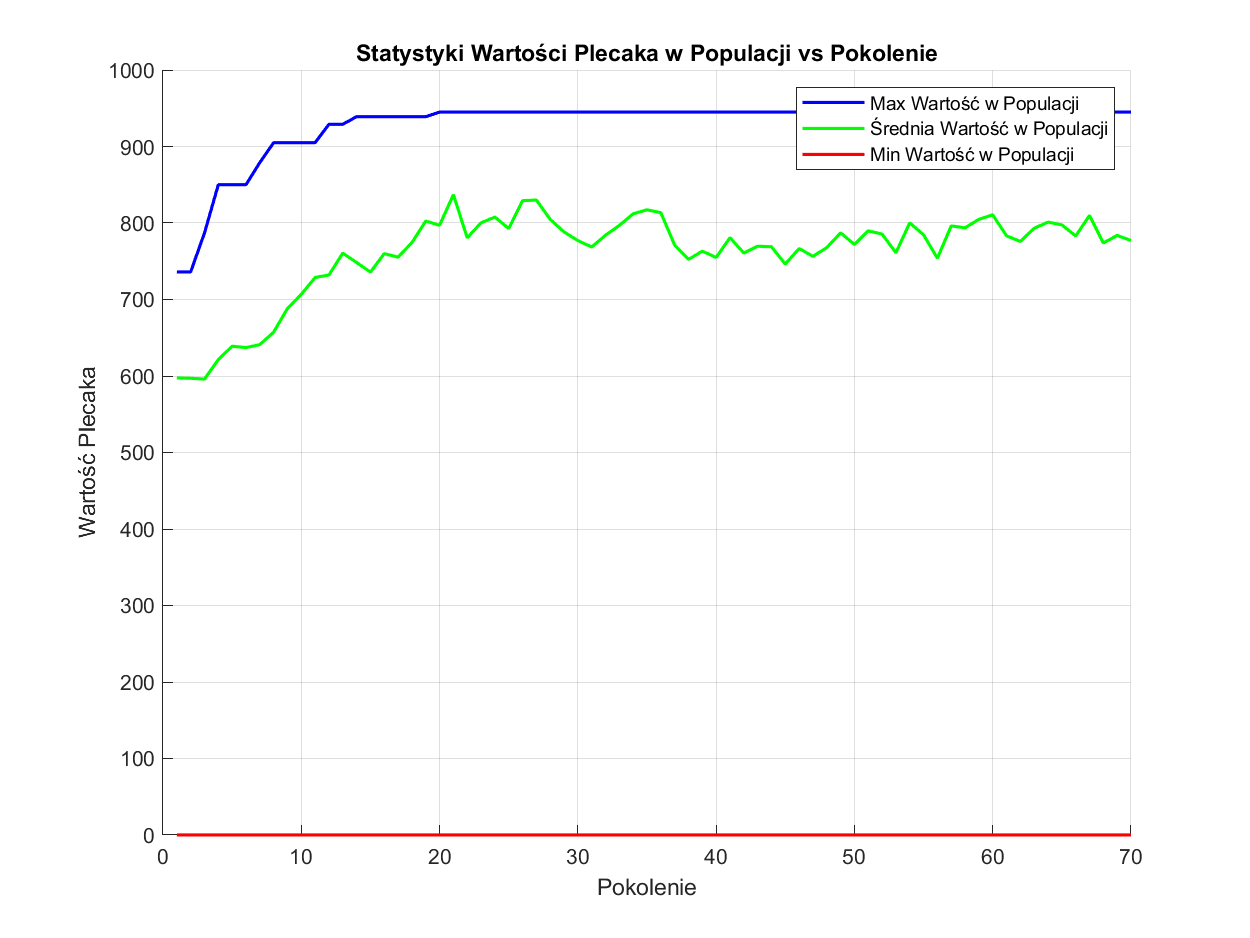
\includegraphics[width=0.9\textwidth]{statistics_plot.png}
    \caption{Statystyki wartości funkcji celu (Max, Średnia, Min) w populacji w zależności od numeru pokolenia. Wartości na wykresie są rzeczywistymi wartościami plecaka (po odwróceniu minimalizacji).}
    \label{fig:stats_plot}
\end{figure}

\begin{figure}[H]
    \centering
    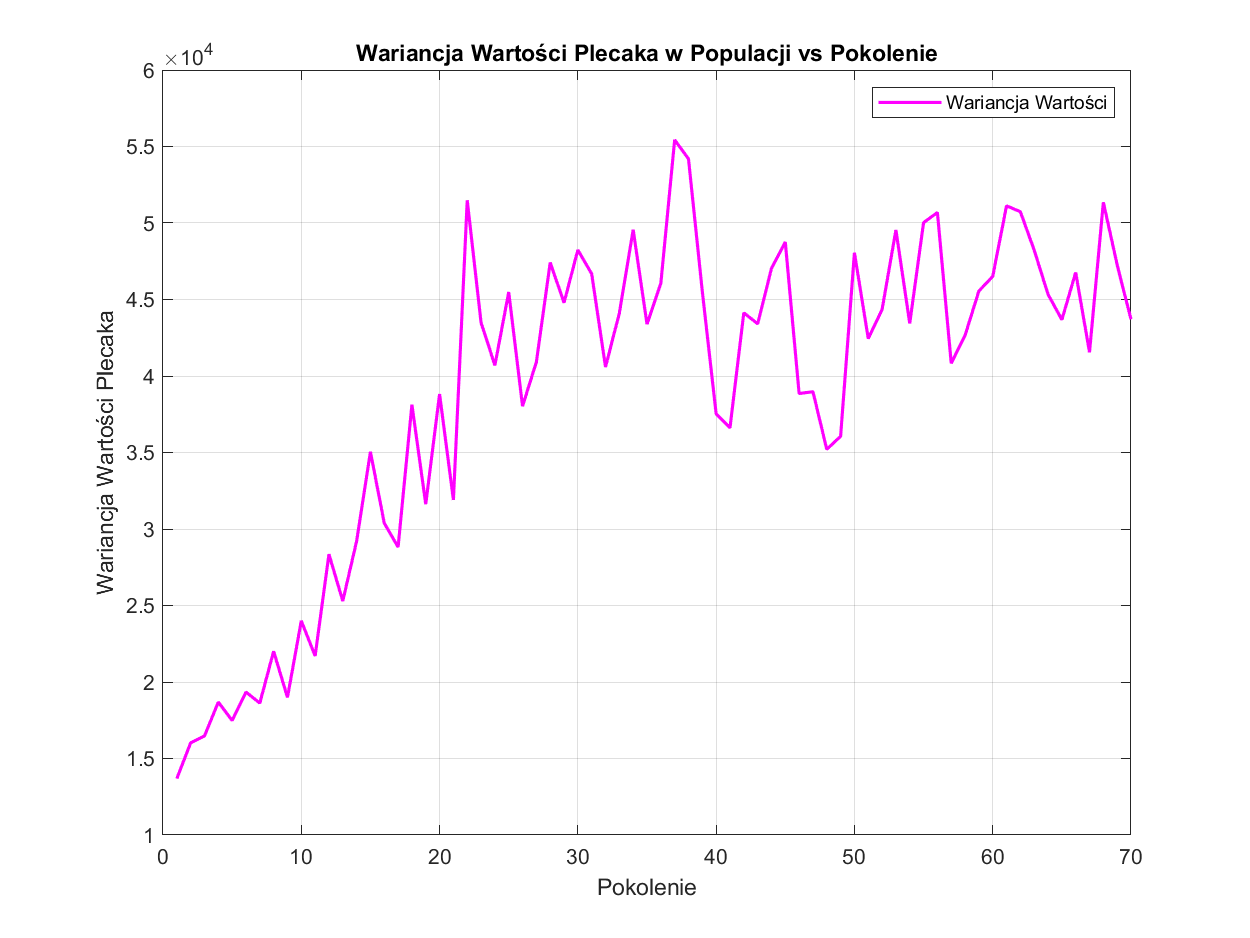
\includegraphics[width=0.9\textwidth]{variance_plot.png}
    \caption{Wariancja wartości funkcji celu w populacji w zależności od numeru pokolenia.}
    \label{fig:variance_plot}
\end{figure}

\newpage
\section{Wnioski}
Algorytm genetyczny zaimplementowany w środowisku MATLAB okazał się skutecznym narzędziem do rozwiązania problemu plecakowego. Uzyskane rozwiązanie maksymalizuje wartość przedmiotów w plecaku, przestrzegając jednocześnie zadanego ograniczenia wagowego.
\begin{itemize}
    \item Znalezione rozwiązanie o łącznej wartości 945 i wadze 5.20 mieści się w dopuszczalnym limicie wagowym 5.22.
    \item Wykresy statystyk funkcji celu (Rysunek \ref{fig:stats_plot}) pokazują zbieżność algorytmu – średnia i maksymalna wartość funkcji celu w populacji rosną w kolejnych pokoleniach, stabilizując się w późniejszych fazach ewolucji.
    \item Wykres wariancji (Rysunek \ref{fig:variance_plot}) ilustruje zmniejszanie się różnorodności populacji w miarę postępu algorytmu, co jest typowe dla procesów ewolucyjnych dążących do optymalnego rozwiązania.
\end{itemize}
Zastosowane parametry algorytmu genetycznego pozwoliły na znalezienie dobrego jakościowo rozwiązania. Dalsze badania mogłyby obejmować analizę wrażliwości algorytmu na zmiany parametrów oraz porównanie z innymi metodami selekcji czy operatorami genetycznymi w celu potencjalnej dalszej optymalizacji wyników.

\end{document}